\chapter{Analyse des Kontrollkanals}
\label{chap:4}
%
Ziel dieser Analyse ist es die benötigten Größen zur Bestimmung einer Normierungskonstante $\alpha$ für den Signalzerfall $\signal$ zu ermitteln. Dazu wird eine schnittbasierte Selektion des Kontrollkanals $\kontroll$ durchgeführt um über die Ermittlung der rekonstruierten Signalkandidaten und der dabei auftretenden Effizienzen die Normierungskonstante bestimmen zu können. Diese ist in Gleichung~\ref{eq:konst} definiert.
%
\begin{equation}
  \alpha=\frac{\mathcal{B}(\kontroll)}{N_{\kontroll}}\frac{(\epsilon_{\text{ges}})_{\kontroll}}{(\epsilon_{\text{ges}})_{\signal}}
  \label{eq:konst}
\end{equation}
%
Hierbei ist~$\mathcal{B}(\kontroll)$ das bereits vermessene Verzweigungsverhältnis des Kontrollkanals ($\SI{5,986(33)}{\percent}$ \cite{pdg}) und~$N_{\kontroll}$ die in dieser Arbeit bestimmte Anzahl der gemessenen Signalereignisse des Normierungskanals.
$\epsilon_{\text{ges}}$ beschreibt die Gesamteffizienzen der Analyse des jeweiligen Kanals. Sie beinhalten die Detektion, Rekonstruktion und Selektion. Die Normierungskonstante ermöglicht es, systematische Fehler in der Bestimmung der Signalkandidaten und Effizienzen des Signalzerfalls $\signal$ möglichst herauszukürzen und so ein deutlich exakteres Ergebnis zu generieren.

\section{Datensätze}
%
Bei dem für die Analyse des Zerfalls $\kontroll$ verwendeten Datensatz handelt es sich um im Jahre 2012 am LHCb-Experiment bei einer integrierten Luminosität von $\SI{2}{\femto\barn^{-1}}$ und einer Schwerpunkstenergie von $\sqrt{s}=\SI{8}{\tera\electronvolt}$ gemessene Daten. Diese wurden neben den am Detektor selbst angewandten Triggern nachträglich selektiert. Dazu ist eine dem Zerfall $\kontroll$ angepasste Selektion (Stripping \texttt{Bu2LLK\_mmLine}) verwendet worden, sodass in dem nTupel noch 8169615 Ereignisse enthalten sind. Davon sind etwa 5959563 real gemessene Daten, sowie etwa 2210052 in sogenannten Monte-Carlo-Simulationen erstellte.\\

Monte-Carlo-Simulationen (MC) stellen eine bewährte Methode dar, um die Physik des Stadardmodells und die real gemessenen Daten vergleichbar zu machen. Um die Vorhersage für das Signal eines bestimmten Zerfalls in Form einer realen Messung anzupassen, werden verschiedene Algorithmen zur Simulierung der Kollisionen sowie deren Messung verwendet. Ziel ist es, die Kollision, anschließende Zerfälle sowie die Wechselwirkungen mit dem spezifischen Detektor möglichst exakt zu simulieren, sodass ein Signaldatensatz entsteht, welcher unter Anderem zur Unterdrückung des real gemssenen Untergrundes, sowie der Suche nach neuer Physik dient. Bei dem hier verwendeten MC werden die Proton-Proton-Kollisionen durch das Programm \texttt{PYTHIA} simuliert, welches über komplexe Modelle die entstehenden Teilchen generiert. Zerfallspunkte sowie die Produkte der bei diesen Kollisionen entstehenden $B$-Mesonen werden durch \texttt{EVTGEN} simuliert. Die anschließende Wechselwirkug der Zerfallsprodukte mit dem Detektor konstruiert der Algorithmus \texttt{GEANT4}, sodass die so entstandenen Datensätze durch dieselbe Hardware und Software (Trigger, rekonstruktion etc.), wie die real am LHCb Gemessenen laufen können. Die Umwandlung der berechneten Ereignisse in die dazu benötigten elektrischen Signale übernimmt die Software \texttt{BOOLE}. Die Simulation geht dabei von einer Schwerpunktsenergie von $\sqrt{s}=\SI{8}{\tera\electronvolt}$ (richtig?) aus. Um die Simulation den Beschaffenheiten des Detektors anzupassen, ist der Winkelbereich der Zerfallsprodukte auf einen etwas größeren als den realen Akzeptanzbereich des Detektors beschränkt. Hierdurch werden Effekte am Rand des Detektors vernachlässigbar.

\section{Selektion des Kontrollkanals}
%
Die Datensätze für den zu untersuchenden Kontrollkanal $\kontroll$ werden zunächst schnittbasiert selektiert. Es erfolgt also eine Einschränkung auf den physikalisch für den gesuchten Zerfall relevanten Bereich. Dazu werden die in Tabelle~\ref{tab:strip} aufgeführten Bedingungen an die relevanten Ereignisse in dem nTupel sowohl an die Daten, als auch an die MC gestellt. Diese Selektion orientiert sich dabei an der in der Studie zur Signaloptimierung \cite{ba-maik} Angewendeten.

\begin{table}[htb]
  \centering
  \caption{Auf den Datensatz angewendete Selektion. *Diese Variable existiert nur im MC.}
  \begin{tabular}{lc}
    \toprule
    Strippingvariable                 & Bedingung      \\
    \midrule
    \texttt{Psi\_MM}                  & $>\num{2946}<\num{3176}$  \\
    \texttt{muminus\_IPCHI2\_OWNPV}   & $>\num{36}$  \\
    \texttt{muplus\_IPCHI2\_OWNPV}    & $>\num{36}$  \\
    \texttt{muminus\_TRACK\_GhostProb}& $<\num{0.3}$ \\
    \texttt{muplus\_TRACK\_GhostProb} & $<\num{0.3}$ \\
    \texttt{Psi\_BKGCAT*}             & $==\num{0}$  \\
    \texttt{Psi\_DIRA\_OWNPV}         & $>\num{0}$  \\
    \bottomrule
  \end{tabular}
  \label{tab:strip}
\end{table}

Ziel dieser Selektion ist es, bei möglichst hoher Effizienz auf tatsächlich aus dem untersuchten Zerfall stammenden Ereignissen, möglichst viele Ereignisse aus sogennanten Untergrund-Zerfällen auszuschließen. Der bei allen Messungen unweigerlich in den Messungen dokumentierte Untergrund stellt eine Kombination verschiedener Teiluntergünde dar. Diese haben mitunter sehr unterschiedliche Ursachen. Der teilweise rekonstruierte Untergrund beispielsweise wird von Zerfällen induziert, die die selben Endprodukte über andere Wege als den gesuchten erreichen. Er überwiegt im unteren Energiebereich. Auch die Fehlerbehaftung der Mesungen der einzelnen Detektorkomponenten erzeugt einen systematischen Untergrund. Einen dritten Beitrag liefert der sogenannte kombinatorische Untergrund, der dadurch entsteht, dass voneinander unabhängige, bei jeder Kollision zwangsläufig über eine weite Energieskala auftretende Prozesse gemessen und fälschlicherweise als Signal identifiziert werden.

Es wird zunächst ein Massenfenster von $m_{\jpsi}=\SI{2946}{\mega\electronvolt}$ bis $m_{\jpsi}=\SI{3176}{\mega\electronvolt}$ um die Masse des $\jpsi$-Mesons gelegt. Diese invariante Masse wird aus den Viererimpulsen der beiden Tochtermyonen berechnet, sodass durch das Fenster sichergestellt wird, dass diese auch aus einem $\jpsi$-Zerfall stammen. Die anderen Selektionsbedingungen sind aus einer rekursiven Optimierung des Signalzerfalls $\signal$ aus der parallel durchgeführten Studie \cite{ba-maik} übernommen, um eine optimale Vergleichbarkeit zu gewährleisten. Selbstverständlich sind sie für den Zerfall $\kontroll$ an die beiden Myonen angepasst. Die Bedingungen \texttt{mu\pm\_IPCHI2\_OWNPV} geben an, wie gut die rekonstruierten Myonen einem Primärvertex zugeordnet werden können. Die Variable \texttt{mu\pm\_TRACK\_GhostProb} gibt an, wie groß die Wahrscheinlichkeit ist, dass die Identifikation eines Myons fälschlicherweise stattfand, sodass die Selektion diese Wahrscheinlichkeit auf maximal $\SI{30}{\percent}$ beschränkt. [andere beiden Variablen] Die Effizienz des so gewählten Strippings auf den MC, sowie den gemssenen Daten berechnet sich nach Gleichungen~\ref{eq:eff_strip1} und \ref{eq:eff_strip2}.
%
\begin{equation}
  \epsilon_\text{strip, MC}=\frac{N_\text{MC-events after stripping}}{N_\text{MC-events}}=\frac{1814293}{2210052}=\SI{82.09}{\percent}
  \label{eq:eff_strip1}
\end{equation}
\begin{equation}
  \epsilon_\text{strip, DATA}=\frac{N_\text{DATA-events after stripping}}{N_\text{DATA-events}}=\frac{2032228}{5959563}=\SI{34.1}{\percent}
  \label{eq:eff_strip2}
\end{equation}
%
Des Weiteren werden sogenannte Triggerstufen als Bedingung für die Selektion der relevanten Ereignisse herangezogen. Die Trigger fungieren als Entscheidungskriterien dafür, ob ein Ereignis potentiell interessante Physik bereithält und somit vom Detektor aufgenommen und gespeichert werden soll, oder nicht. Die \texttt{TOS}-Trigger (\textit{triggered on signal}) lösen dabei aus, wenn Teilchen aus Signalzerfällen detektiert werden. Die hier, sowie in der Signalanalyse \cite{ba-maik} verwendeten Trigger gliedern sich in die in Tabelle~\ref{tab:trigger} aufgeführten drei Stufen \texttt{L0}, \texttt{HLT1} und \texttt{HLT2}. Diese sortieren nacheinander Ereignisse heraus, die nicht mindestens eine der aufgeführten Bedingungen innerhalb einer Stufe erfüllen. Daher selektiert jede Stufe feiner als die Vorherige.
%
\begin{table}[htb]
  \centering
  \caption{Auflistung der verwendeten Trigger.
  Ereignisse, die nicht innerhalb jeder einzelnen Triggerstufe mindestens eine Triggerbedingung erfüllen, werden aussortiert.}
  \begin{tabular}{l}
    \toprule
    \textbf{L0-Trigger}                                           \\
    \quad\texttt{Psi\_L0MuonDecision\_TOS}\quad$==1$              \\
    \quad\texttt{Psi\_L0HadronDecision\_TOS}\quad$==1$            \\
    \quad\texttt{Psi\_L0ElectronDecision\_TOS}\quad$==1$          \\
    \midrule
    \textbf{HLT1-Trigger}                                         \\
    \quad\texttt{Psi\_Hlt1TrackAllL0Decision\_TOS}\quad$==1$      \\
    \quad\texttt{Psi\_Hlt1TrackMuonDecision\_TOS}\quad$==1$       \\
    \midrule
    \textbf{HLT2-Trigger}                                         \\
    \quad\texttt{Psi\_Hlt2Topo2BodyBBDTDecision\_TOS}\quad$==1$   \\
    \quad\texttt{Psi\_Hlt2Topo3BodyBBDTDecision\_TOS}\quad$==1$   \\
    \quad\texttt{Psi\_Hlt2Topo4BodyBBDTDecision\_TOS}\quad$==1$   \\
    \quad\texttt{Psi\_Hlt2TopoMu2BodyBBDTDecision\_TOS}\quad$==1$ \\
    \quad\texttt{Psi\_Hlt2TopoMu3BodyBBDTDecision\_TOS}\quad$==1$ \\
    \quad\texttt{Psi\_Hlt2TopoMu4BodyBBDTDecision\_TOS}\quad$==1$ \\
    \bottomrule
  \end{tabular}
  \label{tab:trigger}
\end{table}
%
Die Effizienz dieser drei Triggerstufen, sowie des Strippings bezogen auf die Zahl der Ereignisse im nTupel beträgt für die Daten und die MC die in den Gleichungen~\ref{eq:eff_ges1} und \ref{eq:eff_ges2} aufgeführten Werte.
%
\begin{equation}
  \epsilon_\text{ges, MC}=\frac{N_\text{MC-events after trigger}}{N_\text{MC-events after stripping}}=\frac{1345240}{2210052}=\SI{60.87}{\percent}
  \label{eq:eff_ges1}
\end{equation}
\begin{equation}
  \epsilon_\text{ges, DATA}=\frac{N_\text{DATA-events after trigger}}{N_\text{DATA-events after stripping}}=\frac{1395768}{5959563}=\SI{23.42}{\percent}
  \label{eq:eff_ges2}
\end{equation}
%
\section{Massenfit}
%
Um aus dem so eingeschränkten und selektierten MC-Datensatz die Anzahl der Signalkandidaten $N_{\kontroll}$ zu bestimmen, wird ein sogennanter \textit{extended maximum-likelihood-fit} der rekonstruierten $\jpsi$-Masse durchgeführt. Die oben beschriebene Selektion beschränkt den Massenbereich des rekonstruierten $\jpsi$-Mesons auf einen Bereich von etwa $[m_{\jpsi}-\SI{150}{\mega\electronvolt}, m_{\jpsi}+\SI{80}{\mega\electronvolt}]$, was der in Abbildung~\ref{fig:mass} dargestellten Verteilung entspricht. Diese Einschränkung konzentriert den fit auf die $\SI{60.87}{\percent}$ der gesamten Ereignisse, welche in diesem Bereich liegen. Gleichzeitig ist das Intervall weit genug gewählt, um auch den eingangs dieses Kapitels beschriebenen Untergrund modellieren zu können.
%
\begin{figure}[H]
  \centering
      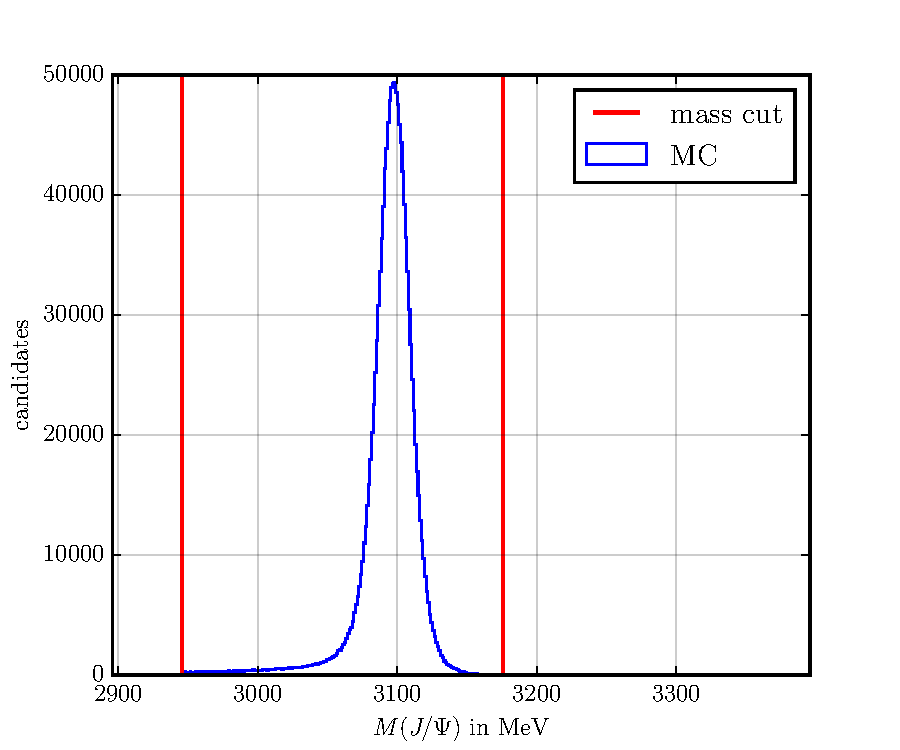
\includegraphics[width=\textwidth]{Plots/jpsi_mass.pdf}
  \caption{Verteilung der $\jpsi$-Masse nach Anwenden der Selektion sowie der Trigger.}
  \label{fig:mass}
\end{figure}
%
Mit Hilfe des Programmes \texttt{RooFit} wird diese Massenverteilung an ein aus Signalmodell und Untergundmodell bestehendes Gesamtmodell angepasst. Dazu wird eine Funktion der in Gleichung~\ref{eq:massenfit} dargestellten Form an die Messpunkte gefittet.
%
\begin{align}
  \symup{G}(m_{\jpsi})=&\; \symup{S}(m_{\jpsi}) + \symup{B}(m_{\jpsi})\\
  \label{eq:massenfit}
  \symup{S}(m_{\jpsi})=&\; \symup{CB}_1(m_{\jpsi},\mu_1,\sigma,\alpha_1,n_1)+f\symup{CB}_2(m_{\jpsi},\mu_2,\sigma,\alpha_2,n_2) \\
  \symup{B}(m_{\jpsi})=&\; e^{\beta\cdot m_{\jpsi}}
\end{align}
%
Hier entspricht die Funktion $\symup{S}(m_{\jpsi})$ dem verwendeten Signalmodell, während $\symup{B}(m_{\jpsi})$ den Hintergund modellieren soll. Das Signalmodell besteht dabei aus zwei sogenannten \textit{Crystal Ball}-Funktionen (CB). Diese zur Modellation asymmetrischer Wahrscheinlichkeitsverteilungen verwendete Funktionen stellen eine Verbindung aus einer Gaußfunktion, welche an einer Seite in eine Potenzfunktion übergeht. Dies ermöglicht die Rekonstruktion sogenannter \textit{tails}, also am Rande einer Gaußfunktion potentiell abfallender Verteilungen. Die analytische darstellung ist in Gleichung~\ref{eq:cb} angegeben.
%
\begin{equation}
  {\displaystyle CB(x;\alpha ,n,{\mu},\sigma,N)=N\cdot {\begin{cases}\exp \left(-{\frac {(x-{\mu})^{2}}{2\sigma ^{2}}}\right),&{\mbox{falls }}{\frac {x-{\mu}}{\sigma }}>-\alpha \\A\cdot \left(B-{\frac {x-{\mu}}{\sigma }}\right)^{-n},&{\mbox{falls }}{\frac {x-{\mu}}{\sigma }}\leqslant -\alpha \end{cases}}}
  \label{eq:cb}
\end{equation}
%
Das Signalmodell wird über insgesamt acht verschiedene Parameter an die Massenverteilung gefittet. Jede CB-Funktion wird dabei über einen eigenen der in Tabelle~\ref{tab:params} aufgeführten Parameter an die Verteilung gefittet.
%
\begin{table}[htb]
  \centering
  \caption{Auflistung der für den fit des Signalmodells verwendeten Parameter.}
  \begin{tabular}{cc}
    \toprule
    \textbf{Crystall Ball 1}    & \textbf{Crystall Ball 2} \\
    \midrule
    $\alpha_1$                  & $\alpha_2$  \\
    $\mu_1$                     & $\mu_2$     \\
    $\sigma$                    & $\sigma$    \\
    $n_1$                       & $n_2$       \\
    $N$                         & $N$         \\
    \bottomrule
  \end{tabular}
  \label{tab:params}
\end{table}
%
$\alpha$ gibt dabei an, ab wann die Gaußglocke durch den Potenzzusammenhang ersetzt wird. $\mu$ beschreibt den
